\section{Durchführung}
\label{sec:Durchführung}

Der Lock-In-Verstärker ist in Abbildung (3) dargestellt.

\begin{figure}[H]
  \centering
  \includegraphics[height=8cm]{verstärker.png}
  \caption{Ein Lock-In-Verstärker und seine Bestandteile.  \cite[S. 3]{l}}
\end{figure}

\noindent Bestandteile sind Vorverstärker, Hoch-, Tief- und Bandpassfilter, Phasenverschieber, Funktionsgenerator, Rauschgenerator, Tiefpass-Verstärker und der Lock-In-Detektor.
Ein Oszilloskop zeigt alle Signale an. 

\noindent Zuerst wird eine wie in Abbildung (4) dargestellte Schaltung aufgebaut. Der Noise Generator wird auf OFF gestellt.
Es wird überprüft, bei welchem Ausgang man die Spannung varrieren kann, und an welchem sie konstant ist.
Als nächstes wird ein sinusförmiges Signal eingestellt und der Ausgang mit einem Referenzsignal, welches auch ein Sinussignal ist, gemischt.
Die Frequenz der beiden Spannungen ist identisch. Insgesamt werden für 5 verschiedene Phasen die Ausgangssignale am Oszilloskop skizziert.
Anschließend wird der Tiefpass hinzugeschaltet und es werden wieder die Spannungen abgegriffen.
Die Ausgangsspannung wird mindestens 10 mal in Abhängigkeit der Phasenverschiebung gemessen.
Die gleiche Messung führt man noch einmal durch, diesmal mit eingeschaltetem Noise Generator.

\begin{figure}[H]
  \centering
  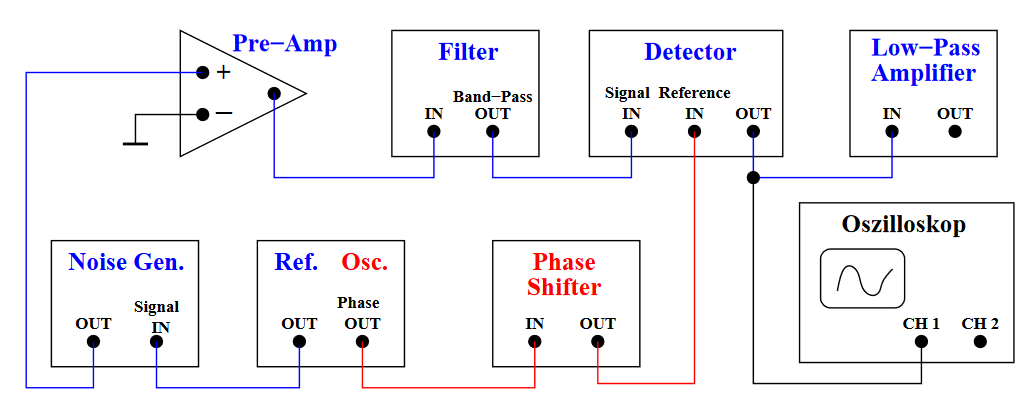
\includegraphics[height=5cm]{aufbau1.png}
  \caption{Schaltung zum ersten Versuchsteil.  \cite[S. 4]{l}}
\end{figure}

\noindent Zuletzt wird eine Photodetektorschaltung wie in Abbildung (5) aufgebaut. 
Es wird die Lichtintensität der LED als Funktion des Abstandes zwischen Diode und LED bestimmt. 
Die Spannung der LED wird mit einer Rechteckspannung moduliert.
Der Abstand wird immer um 5 cm verändert, und es wird solange gemessen, bis die Spannung nicht mehr gemessen werden kann.

\begin{figure}[H]
  \centering
  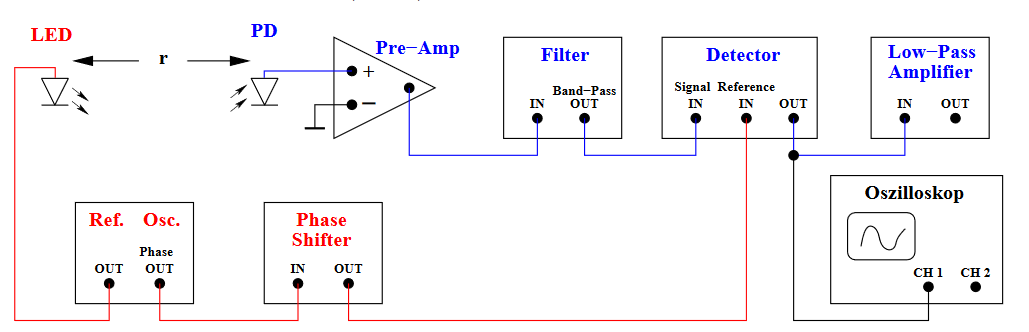
\includegraphics[height=5cm]{aufbau2.png}
  \caption{Photodetektorschaltung zum letzten Versuchsteil.  \cite[S. 5]{l}}
\end{figure}
